\documentclass{standalone}
\usepackage{tikz}
\usepackage{mathrsfs}
\usetikzlibrary{arrows}
\usepackage{xcolor}
\definecolor{forestgreen}{RGB}{34,139,34}
\definecolor{rvwvcq}{rgb}{0.08235294117647059,0.396078431372549,0.7529411764705882}

\begin{document}
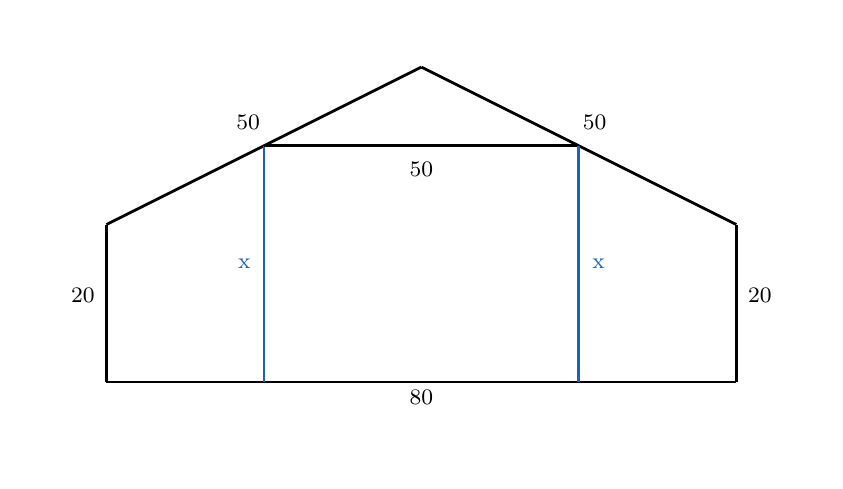
\begin{tikzpicture}[cross/.style={draw, cross out, minimum size=2*(#1-1pt), inner sep=0pt, outer sep=0pt},x=1cm,y=1cm,>=latex,font=\footnotesize,scale=1]
\clip(-5,-1) rectangle (5,4.5);
\draw [line width=1pt] (-4,0)-- (-4,2);
\draw [line width=1pt] (-4,2)-- (0,4);
\draw [line width=1pt] (0,4)-- (4,2);
\draw [line width=1pt] (4,2)-- (4,0);
\draw [line width=1pt] (4,0)-- (-4,0);
\draw [line width=1pt,color=rvwvcq] (-2,0)-- (-2,3);
\draw [line width=1pt] (-2,3)-- (2,3);
\draw [line width=1pt,color=rvwvcq] (2,3)-- (2,0);
\begin{scriptsize}
    \draw[color=black] (-4.3,1.1) node {20};
    \draw[color=black] (-2.2,3.3) node {50};
    \draw[color=black] (2.2,3.3) node {50};
    \draw[color=black] (4.3,1.1) node {20};
    \draw[color=black] (0,-0.2) node {80};
    \draw[color=rvwvcq] (-2.25,1.5) node {x};
    \draw[color=black] (-0,2.7) node {50};
    \draw[color=rvwvcq] (2.25,1.5) node {x};
\end{scriptsize}
\end{tikzpicture}


\end{document}